%%
%% This is file `lexample.tex', 
%% Sample file for siam macros for use with LaTeX 2e
%% 
%% October 1, 1995
%%
%% Version 1.0
%% 
%% You are not allowed to change this file. 
%% 
%% You are allowed to distribute this file under the condition that 
%% it is distributed together with all of the files in the siam macro 
%% distribution. These are:
%%
%%  siamltex.cls (main LaTeX macro file for SIAM)
%%  siamltex.sty (includes siamltex.cls for compatibility mode)
%%  siam10.clo   (size option for 10pt papers)
%%  subeqn.clo   (allows equation numbners with lettered subelements)
%%  siam.bst     (bibliographic style file for BibTeX)
%%  docultex.tex (documentation file)
%%  lexample.tex (this file)
%%
%% If you receive only some of these files from someone, complain! 
%% 
%% You are NOT ALLOWED to distribute this file alone. You are NOT 
%% ALLOWED to take money for the distribution or use of either this 
%% file or a changed version, except for a nominal charge for copying 
%% etc. 
%% \CharacterTable
%%  {Upper-case    \A\B\C\D\E\F\G\H\I\J\K\L\M\N\O\P\Q\R\S\T\U\V\W\X\Y\Z
%%   Lower-case    \a\b\c\d\e\f\g\h\i\j\k\l\m\n\o\p\q\r\s\t\u\v\w\x\y\z
%%   Digits        \0\1\2\3\4\5\6\7\8\9
%%   Exclamation   \!     Double quote  \"     Hash (number) \#
%%   Dollar        \$     Percent       \%     Ampersand     \&
%%   Acute accent  \'     Left paren    \(     Right paren   \)
%%   Asterisk      \*     Plus          \+     Comma         \,
%%   Minus         \-     Point         \.     Solidus       \/
%%   Colon         \:     Semicolon     \;     Less than     \<
%%   Equals        \=     Greater than  \>     Question mark \?
%%   Commercial at \@     Left bracket  \[     Backslash     \\
%%   Right bracket \]     Circumflex    \^     Underscore    \_
%%   Grave accent  \`     Left brace    \{     Vertical bar  \|
%%   Right brace   \}     Tilde         \~}

\documentclass[final,leqno]{siamltex}
%\newcommand\floor[1]{\lfloor#1\rfloor}
\usepackage{amsmath}
\usepackage{svg}
\usepackage{graphicx}
% definitions used by included articles, reproduced here for 
% educational benefit, and to minimize alterations needed to be made
% in developing this sample file.

\usepackage{caption}
\usepackage{subfig}
\usepackage{pdflscape}

\usepackage{mathtools}
\DeclarePairedDelimiter\floor{\lfloor}{\rfloor}

\newcommand{\pe}{\psi}
\def\d{\delta} 
\def\ds{\displaystyle} 
\def\e{{\epsilon}} 
\def\eb{\bar{\eta}}  
\def\enorm#1{\|#1\|_2} 
\def\Fp{F^\prime}  
\def\fishpack{{FISHPACK}} 
\def\fortran{{FORTRAN}} 
\def\gmres{{GMRES}} 
\def\gmresm{{\rm GMRES($m$)}} 
\def\Kc{{\cal K}} 
\def\norm#1{\|#1\|} 
\def\wb{{\bar w}} 
\def\zb{{\bar z}} 

% some definitions of bold math italics to make typing easier.
% They are used in the corollary.

\def\bfE{\mbox{\boldmath$E$}}
\def\bfG{\mbox{\boldmath$G$}}

\title{Evaluating a sublinear-time algorithm for the minimum spanning tree weight problem}

% The thanks line in the title should be filled in if there is
% any support acknowledgement for the overall work to be included
% This \thanks is also used for the received by date info, but
% authors are not expected to provide this.

\author{Gabriele Santi\thanks{Master's Degree in Computer Science, University of Rome ``Tor Vergata'' ({\tt gabriele.santi@acm.org}).}
        \and Leonardo De Laurentiis\thanks{Master's Degree in Computer Science, University of Rome ``Tor Vergata'' ({\tt ldelaurentiis@acm.org}).}}

\begin{document}

\maketitle

\begin{abstract}
We present an implementation and an experimental evaluation of an algorithm that, given a connected graph G (represented by adjacency lists), estimates in sublinear time, with a relative error $e$, the Minimum Spanning Tree Weight of G (see~\cite{crt} for a theoretical exposure of the algorithm). 
Since the theoretical performances have already been shown and demonstrated in the above-mentioned paper of Chazelle et al. our goal is, exclusively, to experimental evaluate the algorithm and at last to present the results.
Some technical insights are given on the implementation of the algorithm and on the dataset used in the test phase, hence to show how the experiment has been led out even for reproducibility purposes;
the results are then evaluated empirically and widely discussed, comparing these with the performances of the Prim algorithm and the Kruskal algorithm, launching several runs on a heterogeneous set of graphs and different theoretical models for them.

We assume hereafter that the reader has knowledge about the cited paper as we will just recap the theoretical results.
\end{abstract}

\begin{keywords} 
minimum spanning tree, sublinear time algorithms, randomized algorithm, approximation algorithm, minimum spanning tree weight, experimental evaluation 
\end{keywords}

\begin{AMS}
68W20, 68W25, 68R10
\end{AMS}

\pagestyle{myheadings}
\thispagestyle{plain}
\markboth{GABRIELE SANTI AND LEONARDO DE LAURENTIIS}{EVALUATING A SUBLINEAR-TIME ALGORITHM FOR THE MST WEIGHT PROBLEM}


\section{Introduction}
%We would discuss here some preliminary observations and assumptions. First of all, we observe that we need a set of connected graphs represented in a homogeneous manner, and in the form of adjacency lists, as the same paper says. The graphs and their representations which can easily be found (e.g. on the Internet) are too hetereogeneous, and there is some difficulty to find a good homogeneous (i.e. represented in the same format) set of connected graphs.

We would discuss here some preliminary observations and assumptions. First of all, we observe that we need a set of graphs that satisfies the following points:
\begin{itemize}
 \item they should be finite and should not be multigraphs;
 \item they should be undirected;
 \item they should have weighted edges;
 \item the weights on the edges should be integers; since the graph is finite, it is enough to show that there exist $W$ such that it is the maximum weight on the edges of the graph;\footnote{more generally, it is enough to have a numerable set of values for the weights which is always true when the graph is finite}
 \item they might contain self-loops;
 \item they have to be connected (the graph has only one connected component);
 \item they should be represented with adjacency lists;
 \item they should be represented in the same manner (we need an unvarying file format).
\end{itemize}
Unfortunately, the graphs and their representations which can easily be found on the Internet doesn't accomplish all of this requirements at the same time, although many standards for the file format are available.

Given this observation, our choice was to use randomly generated graphs, hence to implement our own graphs generator. This gives us the opportunity to generate a wide set of connected graphs, with tunable parameters, carefully chosen looking forward to the tests; these parameters include the number of nodes, the number of edges and the edges weight, nonetheless the distribution law for the edges. The edges between the nodes are step-by-step randomly constructed, respecting the connection requirement. The different types of graphs that we use in our experimental evaluation are presented afterwards.

After studying the paper we made some assumptions. One of the problem we encountered is that the theoretical algorithm assume to have in input the graph $G$ and to have direct access to the family of graphs $G_i$\footnote{we recall that $G_i$ is an induced subgraph of $G$ such that the maximum weight on his edges is $i$ (e.g. $G_w$ is exactly $G$)}; with ``direct'' we intend that no computation is required to extract $G_i$, which is not true. In fact, we can show easily that a lower bound for the extraction of all the family costs at least $O(m)$ (i.e. is linear on the number of edges). A na\"{\i}ve approach would cost $O(m)$ for the extraction of $G_i$ for a given $i$, hence $O(w m)$ for the whole family; a better approach could order the edges in $O(m \log m)$ and build the family in a single pass on the edges, achieving $O(m + m \log m)$. Having in input only $G$ it would seem that the algorithm is responsible for the extraction of the family, but it couldn't be due to this lower bound that would sabotage the overall performance. We decided finally to consider this cost a part of the construction of the data structure of the graph, to be done prior to the call of the algorithm.

%At first, it seems fair to include the computing time for the weight-based subgraphs in the total computing time, since the input of the algorithm is said to be 'G' and not 'G with its subgraphs'. Making a more in-depth analysis, as the same paper says, the aim of the algorithm is to be sublinear in the number of edges (i.e. below $O(m)$, where m is the number of edges of the graph); this gives us the opportunity of a legitimate choice: to keep the time to compute weight-based subgraphs out of the total computing time. This is, in our opinion, a legitimate observation, since the time to compute weight-based subgraphs is at least $O(m)$.

%Another thing that we notice is that the algorithm lends well itself to a parallelized running; for example, we can easily make parallelized the execution of the “approx-MST-weight” routine, using $w-1$ threads. Since a parallel execution is out of scope to prove the algorithm goodness, this observation leads only to a possible future development; in this context, we are only interested in testing the sequential algorithm bound. VA SULLE CONSIDERAZIONI FINALI

 
\section{Design studies and choices} 

\subsection{Random Graphs Generator}
As mentioned before, our choice is to implement our own graphs generator. The aim is to generate \emph{connected random graphs} with a specific set of parameters, like the number of nodes, the number of edges, the maximum edges weight and the average degree. More, we want to test how our algorithm behaves in different environments, so we want to control the distribution law of the edges. Keep in mind that the graph has to satisfy all the points of the previous section, among which the connectivity requirement. Given a desired number of nodes $n$ and $e \geq n-1$ edges, the key-concepts under the implementation of our connected graphs generator are the following: 
\begin{itemize}
 \item we begin by generating a random permutation of the vertices $v_0, v_1, \dots v_n$
 \item we generate a random spanning tree by iteratively adding edges in this vector in a uniform random manner; suppose we have added $\tau$ vertices to the tree $T$, we randomly select a vertex $s$ in the set $\lbrace T_0, \dots, T_\tau \rbrace$ and add a new edge $<T_s, v_{\tau+1}>$. At the end we will have an acyclic graph with $n-1$ edges.
 \item following a certain probability law, we add the remaining $e - (n-1)$ edges
\end{itemize}
note that every time we add an edge, a weight is associated to it, with a value uniformly choosen in $\left[ 1, w \right]$.

We even decided to use a custom file format to save the data, wich is a \texttt{.ssv} file, which stands for \emph{space separated values}: every line of the file corresponds to two edges, reporting the values $<v_s, v_t, w>$ that means source and target nodes, edge weight. Being the graph undirected, it is implicit that the edge $<v_t, v_s, w>$ exists also.


\subsection{Graph Data Structures}
We implemented two version of the algorithm, the first using the well-known \emph{Boost}'s BGL\footnote{\texttt{Boost Graph Libray}, \cite{bst}} for the graphs data structures and efficient implementations of Kruskal's and Prim's algorithms. The latter uses our own implementation of both the structures and the algorithms. We decided to do so because we wanted more control over the code, for testing purposes, and because at the moment (version \texttt{1.61.0}) the BGL subgraphs framework presents some still unfixed bug.

Unfortunately, our Kruskal algorithm, although using \emph{union-find} structures with path compression\footnote{it is known that the Kruskal algorithm time complexity is $O(m \log m)$, but can be improved to $O(m \log n)$ using union find structures with some euristic conveniently applied}, is not fine-tuned as that proposed by the Boost's libraries; we didn't take further time on this because on the other side, our version of Prim's algorithm shows the \emph{same exact performances} of the Boost version and it counts as lower bound being optimal and way better than the Kruskal solution. Our data structures have been called FastGraph for their optimization over the operation required for the test. In any way our data structures \emph{can} nor \emph{do} ``help'' the CRT\footnote{Short for B. Chazelle, R. Rubinfeld, and L. Trevisan.\cite{crt}} algorithm in improving his time complexity.

\subsection{Tuning the algorithm}
In the implementation of the algorithm, the graph stored in the text file is read in a FastGraph, which is of course a representation by adjacency lists.
We want to compare the performances of CRT algorithm with a standard MST algorithm that in addition computes the total weight.\\
We want to emphasize now that the CRT algorithm is based on probabilistic assumptions; some parameters, that depend asymptotically on $\varepsilon$ should be selected carefully in order to
provide a good approximation very fast. These includes: 
\begin{itemize}
\item $r$, the number of vertices uniformly choosen in the ``approx-number-connected-components''. This number is critical for the performances, as it directly determines the running time of the entire algorithm.
\item $C$, the large costant that we use to pick the number of vertices determinants for the application of the original paper's Lemma 4.
\end{itemize}

Both these values largely affect the overall performances because they undirectly decide how many BFS will be carried out by the CRT algorithm; the BFSes represent the fundamental cost driver of the entire run.

Initially in our opinion, the choice of these parameters must depend on the number of vertices in a way that they are dynamic, keeping their dependency on $\varepsilon$. We tried to untie this bond to $n$ but having static values for this parameters show poor performances and a relative error exploding too fast as we grow the input instance.
 
As the paper says, the only requirement for $r$ is that it is $O(\frac{1}{\varepsilon^{2}})$ and $C \in O(\frac{1}{\varepsilon})$.

The demonstration reported on the original paper bound these values in a way that helped us on choosing the right function to compute them; in fact, we have that\footnote{see Theorem 7 and Theorem 8 of \cite{crt}}
\[
 r \sqrt{\frac{w}{n}} < \varepsilon < 1/2, \qquad \frac{C}{\sqrt{n}} < \varepsilon < 1/2
\]
hence we choose 

\[
 r = \floor*{ \frac{\floor*{ \sqrt{\frac{n}{w}} \varepsilon - 1 }}{\varepsilon^2}} \in O \left( \frac{1}{\varepsilon^2} \right)
\]
\[
 C = \floor*{ \frac{\floor*{ \sqrt{n} \varepsilon - 1}}{\varepsilon}} \in O \left( \frac{1}{\varepsilon} \right)
\]


%Therefore we choose the following function to compute the $r$ parameter: $\floor{\dfrac{{(\sqrt{\dfrac{n}{w}}\cdot \varepsilon)-1}}{\varepsilon^{2}}}$.\\ \\
%Regarding the large constant C, we choose the following function to compute the vertices for the Lemma 4: $\floor{{(\sqrt{n}\cdot \varepsilon)-1}}$; therefore we compute the vertices with the following: $\dfrac{C}{\varepsilon}$.\\

\subsection{Random Sequences}
Another problem we encountered was the random selection of $k$ distinct vertices out of $n$ with $k<n$; after some research, we found that this kind of problem cannot be solved in sublinear time on the number of vertices, which can't be done for the same reasons exposed in the introduction about the subgraph family. The problem here is that we can't extract \emph{with no reinsertion} $k$ values without using an external data structure; this structure has a linear cost for the maintainance that depends on $n$. A special case is represented if $n$ is a prime that fulfills certain properties, in that case we can extract a value in constant time without repetition; this solution is not affordable here because we need a dynamic range for each call.

The solution we found is to use Fisher-Yates sequences\footnote{originally decribed in \cite{fys} and then redesigned for computer use in \cite{fysc}} which permits us to prepare in advance the sequences and then get different, distinct values at each call in constant time and with dynamic bounds. The cost of the preparation is linear and is not considered in the total cost.


\section{Implementation choices}
We choose to implement the algorithm in C++ because we wanted a language that offers the advantages of an OOP language, not least a faster development, that had a standard library and sufficiently ``near'' the machine to have a tighter control over the performances and the memory occupation (e.g. performances high variance due to overhead of a VM or an interpreter). We considered that absolute performances are not important here, whereas relative performances of the CRT algorithm and other MST algorithms are the focus, so finally the choice of the language is something not of the greatest importance. The IDE tool used for the implementation is JetBrains Clion.
We also used GitHub, as our code versioning control system.

Also, as already mentioned, we did use the Boost library to extend the STL that C++ already offers; we did implement FastGraph in place of BGL also to address memory issues in relation to the method Boost uses to store subgraphs of a graph; we in fact used an advanced method to store the family of subgraphs $G_i, i = 0,1,\dots,w$ that simply store the difference of vertices between them, $\Delta_{G_i} := V(G_i) - V(G_{i-1})$. It is always possibile to reconstruct every $G_i$ because this family only has \emph{induced} subgraphs, and this cost is not taken into account in the computation of the total time.\\

The main function of the implementation is in the “AlgoWEB.cpp” file.
Launching the program from this file allows us to run either the CRT algorithm or the Prim algorithm,or the Kruskal algorithm, and to view either the running time or the computed weight of the Minimum Spanning Tree. It takes some argument in input, namely the file containing the graph, a suitable value for $\varepsilon$ and the path where to save the results of the single run.

Besides, it is possible to run the random graph generator by the \texttt{grandom} utility we developed apart. It takes many arguments in input, that you can find just by calling
\begin{verbatim}
 $> grandom -h|--help
\end{verbatim}

\subsection{Random Graphs Models}
In order to give exhaustive results, we designed \texttt{grandom} to produce 4 classes of random graphs:
\begin{itemize}
\item Erd\H{o}s-R\'{e}nyi model, that builds random graphs constructed with a uniform distribution fo the edges and an average degree $d \approx \frac{2m}{n}$;
\item Gaussian model, that builds random graphs with a ``cluster zone'' where the edges are more frequent, hence the gaussian shape of the degree distribution; we have still $d \approx \frac{2m}{n}$;
\item Barab\'{a}si-Albert model, that builds random \emph{scale-free} graphs. The average degree is $d \approx \frac{m}{n}$;
\item Watts-Strogatz model, that builds random graphs with \emph{small-world} properties and $d \approx \frac{2m}{n}$.
\end{itemize}

\section{Tests}
The following section reports the results we had launching the algorithm over a variegate dataset of graphs, as described in the next paragraph.

\subsection{Dataset}
For each random graph model listed in the previous section we decided to produce a dataset; each dataset has a ``family'' of graphs that differs one from each other following a pattern for the parameters. Precisely, this is how the dataset is composed following the rules:
\begin{itemize}
\item build one graph for each model (\textsf{Uniform, Gaussian, Small-World, Scale-Free}):
\item for each selected value of $n$, i.e. the number of nodes ($5000$, $30000$, $55000$, $80000$, $105000$, $130000$, $155000$, $180000$, $205000$, $230000$):
\item for each selected value of $d$, i.e. the average degree ($20, 100, 200$):
\item since we have, for our models and for the fact that $m \propto n$, a proportion between the previous quantity and the number of edges $m$, i.e. $d \, \xrightarrow{n \rightharpoonup + \infty} \, \frac{2m}{n}$, we have the selected values for $m$ ($10, 50, 100$ times $n$)\footnote{operatively we fixed the number of edges, so $d$ is a random variable}:
\item then for each selected value of $w$, i.e. the weight ($20, 40, 60, 80$).
\end{itemize}

Finally we have \textsf{the number of models} $\times$ \textsf{the number of selected values for $n$} $\times$ \textsf{the number of selected values for $d$ (hence $m$)} $\times$ \textsf{the number of selected values for $w$} for a total of $4 \cdot 10 \cdot 3 \cdot 4 = 480$ graphs. This dataset, made of plain text files as already described, is quite heavy: $42.1$ GiB of data. 

\subsection{Runs}

Using the dataset just described, we used a pattern for the runs, in order to have a complete view of the behavior of the algorithm in the domain of the various parameters:
\begin{itemize}
 \item build three plots for each model:
 \item for each selected value of $\varepsilon$ ($0.2, 0.3, 0.4, 0.49999$):
 \item for each selected value of $d/2 \simeq \frac{m}{n}$ ($10, 50, 100$):
 \item for each selected value of $w$.
\end{itemize}

The first two plots report the absolute and relative error of the CRT result compared to the correct one, calculated with Prim's algorithm; the third report the trend of the used time. As we mentioned, we indeed used Kruskal too but it's not reported here for it was not faster than Prim for the times and unuseful for the results.

We had this way a total of $3 \cdot 4 \cdot 3 \cdot 4 = 144$ plots, or better $48$ different cases of study.
As mentioned before, the parameters should be selected carefully in order to provide a good approximation very fast. In this sense $\varepsilon$ plays a crucial role here: since the CRT algorithm is a probabilistic algorithm and $\varepsilon$ is indeed the driver parameter either for performances and for the accuracy of the estimate MST weight, it does not make sense to choose values too small for this parameter, as the performances could dramatically degrades (as, indeed, is expected).
So, although it could be of interest to study the right limit of $1/2$, we empirically noted that values of $\varepsilon$ below $0.2$ shows undesired behaviour of the CRT algorithm, for the results and for the running times either.

Given the intrinsically probabilistic nature of the CRT algorithm, we have to launch several runs on the same graph, to have a correct estimate of the CRT running time. For this purpose we decided to launch 10 runs for each graph of the dataset, and to take the average running time as the estimate of the running time. For the approximated MST weight we instead toke one of them randomly, to preserve the information on the tolerance of the estimate.

 
\section{Results} 
 
Following there are some considerations and some line charts regarding the main results.

We know that the CRT time complexity is $O(dw\varepsilon^{-2} \log{\dfrac{dw}{\varepsilon}})$, where $d$ is the average degree of a graph; indeed we know that the accuracy depends on $\varepsilon$ also, so we expect an inversely proportional relation with the running time. Therefore what we expect is that:\\
\begin{itemize}
\item increase one or more of the parameters $d$, $w$, there should be a worsening of the average running time;
\item keeping all the other parameters unchanged, if we consider an increase in the value of $\varepsilon$ there must be an improvement of the running time (as well as a worsening of the result, though);
\item viceversa we expect the opposite behaviour if we decrease $d$ and/or $w$ or decrease $\varepsilon$ with the other parameters unchanged.
\end{itemize}
Let us call the above \emph{crucial parameters}.

%We also know that the aim of the CRT algorithm is to be sublinear in the number of edges (i.e. below $O(m)$, where m is the number of edges of the graph); we want now to show that it really happens, possibly for all the different types of graphs in our dataset.

First thing to show is that the CRT algorithm is sublinear in the number of edges, hence is better than any other \emph{exact} algorithm. This can be easily seen in figures from~\ref{U_03_50_40_time_kruskal} to~\ref{U_03_50_40_rel}. For the rest of the plots listed from now on, it is possibile to see the values of the parameters for the presented run above the graph.

\begin{figure}[htbp]
 \centering
 \subfloat[][\emph{Running time}.]
 {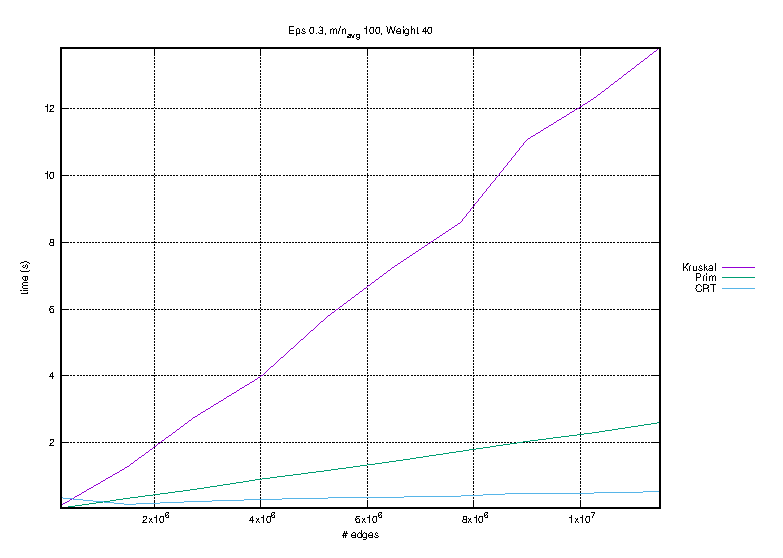
\includegraphics[width=.8\textwidth]{plots/uniform_03_50_40_time_kruskal}\label{U_03_50_40_time_kruskal}} \\
 \subfloat[][\emph{Relative error}.]
 {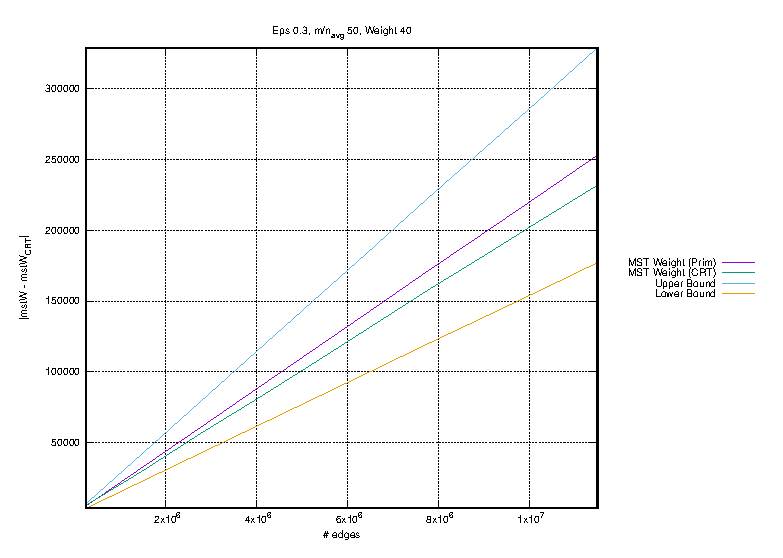
\includegraphics[width=.45\textwidth]{plots/uniform_03_50_40_abs}\label{U_03_50_40_abs}} \quad
 \subfloat[][\emph{Absolute error}.]
 {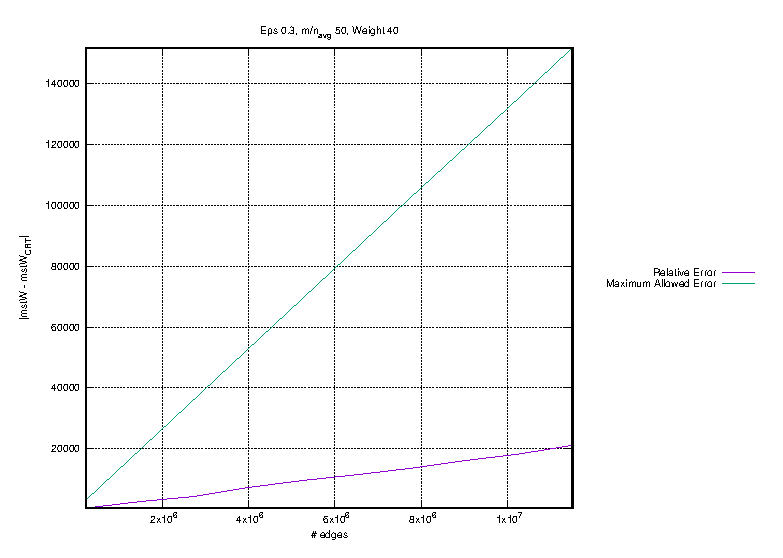
\includegraphics[width=.45\textwidth]{plots/uniform_03_50_40_rel}\label{U_03_50_40_rel}}
 \caption{Sublinearity of the CRT algorithm.}
 \label{is_sublin}
\end{figure}

Given that the CRT Algorithm respects the sub-linearity constraint, let's see the variations that occur when selectively changing other parameters.
  
%At first, we can observe that given fixed values of $d$, $w$ and $\varepsilon$ the CRT Algorithm respects the sub-linearity property, for all the different types of graphs in our dataset, as the reader can see in the figures from~\ref{GAUSSIAN_E_02_W_20_D_10} to~\ref{UNIFORM_E_02_W_20_D_10}.\\

\subsection{Variations of crucial parameters}

\subsubsection{Average degree}
Let us now see the behaviour for the variation of $d$; we will initially concentrate on the running time and solely for the \textsf{uniform} model. The selected values of $\varepsilon$ and $w$ are respectivey $0.3$ and $40$. 

\begin{figure}[htbp]
 \centering
 \subfloat[][$d \simeq 20$]
 {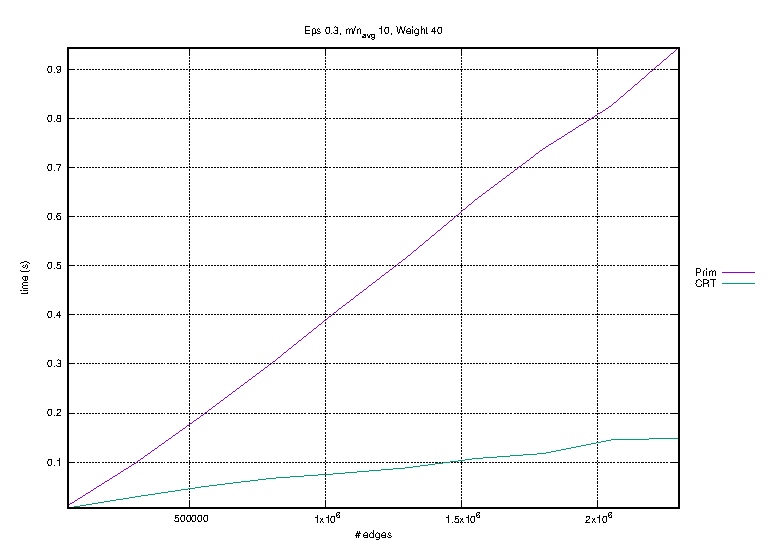
\includegraphics[width=.65\textwidth]{plots/uniform_03_10_40_time}\label{U_03_10_40_time}} \\
 \subfloat[][$d \simeq 100$]
 {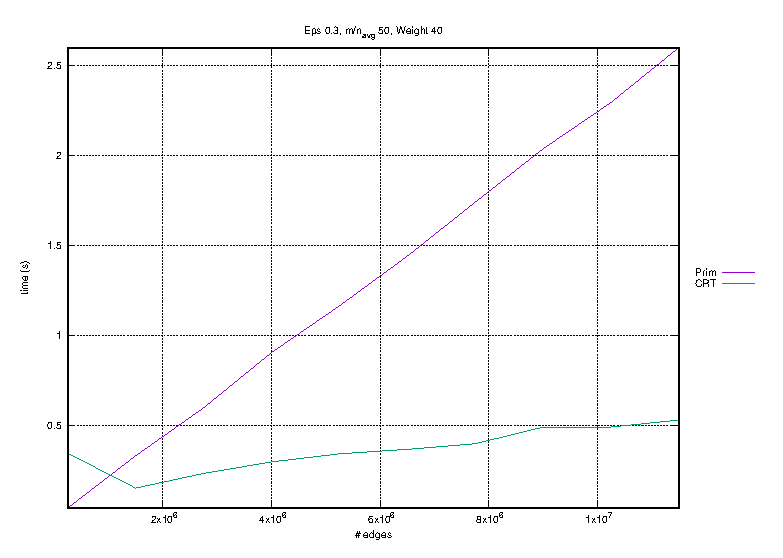
\includegraphics[width=.65\textwidth]{plots/uniform_03_50_40_time}\label{U_03_50_40_time}} \\
 \subfloat[][$d \simeq 200$]
 {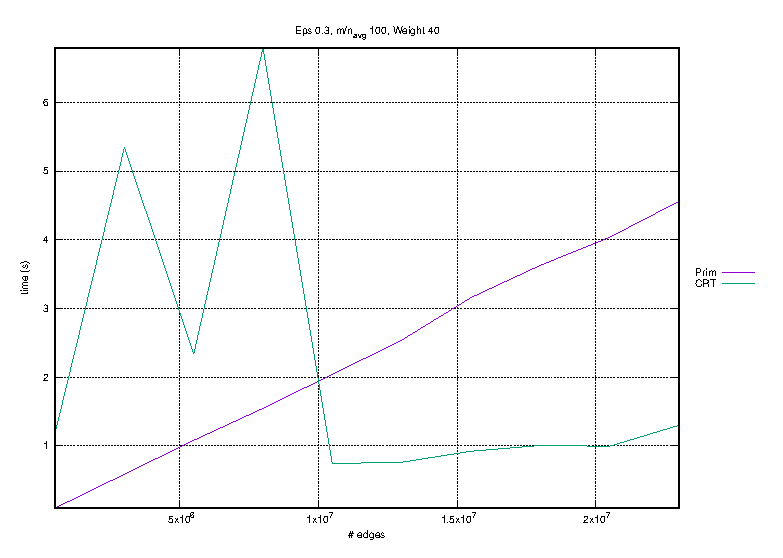
\includegraphics[width=.65\textwidth]{plots/uniform_03_100_40_time}\label{U_03_100_40_time}}
 \caption{Behaviour for the increase of $d$.}
 \label{d_increase}
\end{figure}

As we can see in figures~\ref{U_03_10_40_time} to~\ref{U_03_100_40_time}, there is a worsening in the performance \emph{for small instances}: an increase of the average degree $d$ is somewhat correlated to a loss of performances to the point that our property testing algorithm needs more time that the deterministic one; still, that seems to be true \emph{under} a certain dimension of the instance of the graph, so that we don't lose the truthfulness of the theoretical time complexity because for a fixed $d^*$ it will always be possibile to find empirically a certain number of edges $m^* \propto d^*$ beyond which the running time function is always below $C \cdot dw\varepsilon^{-2} \log{\dfrac{dw}{\varepsilon}}$ for a certain $C$.\footnote{that comes directly from the definition of \emph{asymptotic complexity}}

We would speculate that the error could be related to this. Indeed in figure~\ref{d_increase_rel} we can see 

\begin{figure}[htbp]
 \centering
 \subfloat[][$d \simeq 20$]
 {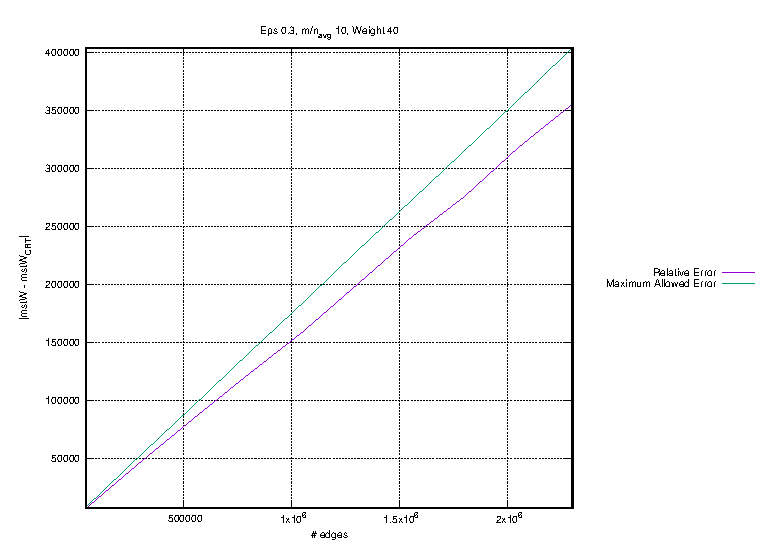
\includegraphics[width=.65\textwidth]{plots/uniform_03_10_40_rel}\label{U_03_10_40_rel}} \\
 \subfloat[][$d \simeq 100$]
 {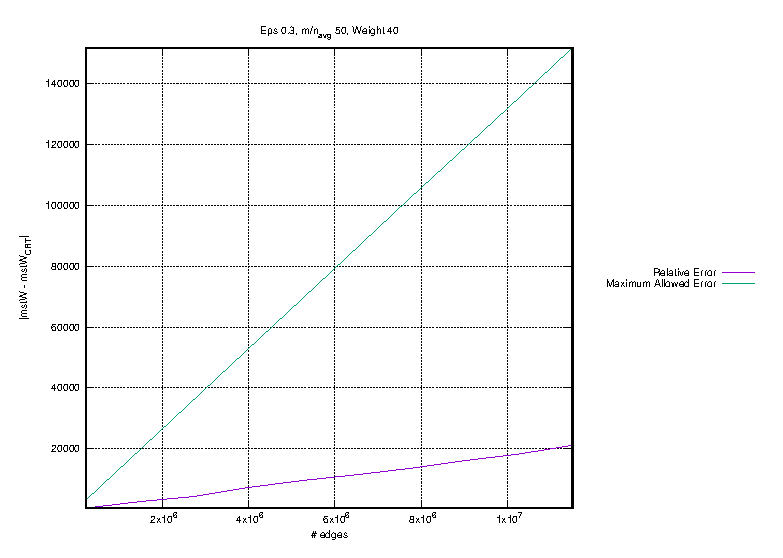
\includegraphics[width=.65\textwidth]{plots/uniform_03_50_40_rel}\label{U_03_50_40_rel2}} \\
 \subfloat[][$d \simeq 200$]
 {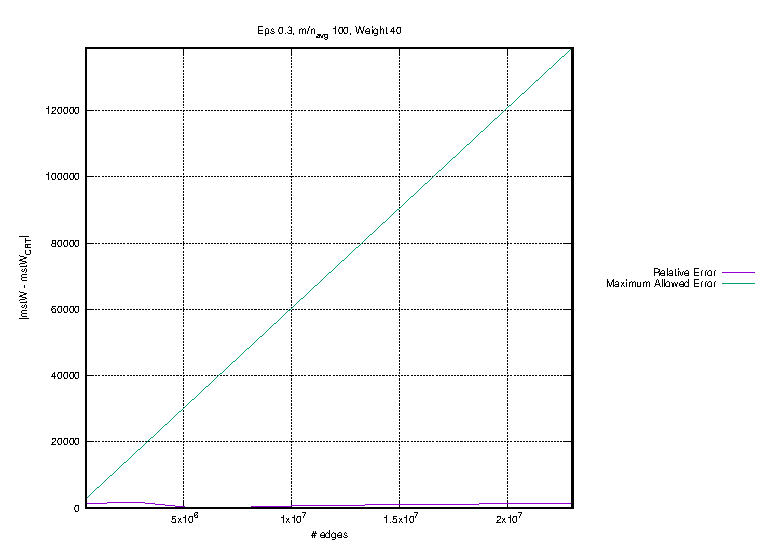
\includegraphics[width=.65\textwidth]{plots/uniform_03_100_40_rel}\label{U_03_100_40_rel}}
 \caption{Behaviour for the increase of $d$.}
 \label{d_increase_rel}
\end{figure}

 
 
\subsection{Variations of graph model}

\begin{landscape}

\begin{figure}[htbp]
 \centering
 \subfloat[][uniform, time trend]
 {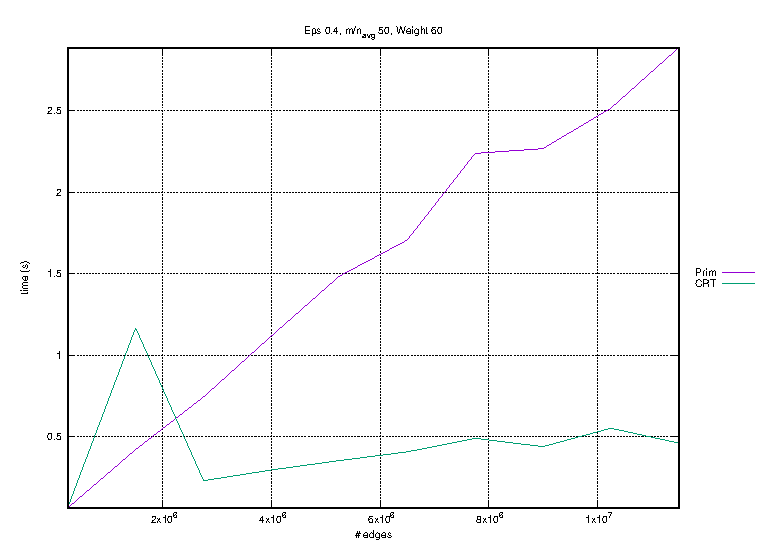
\includegraphics[width=.411\textwidth]{plots/uniform_04_50_60_time}\label{U_04_50_60_time}}
 \subfloat[][gaussian, time trend]
 {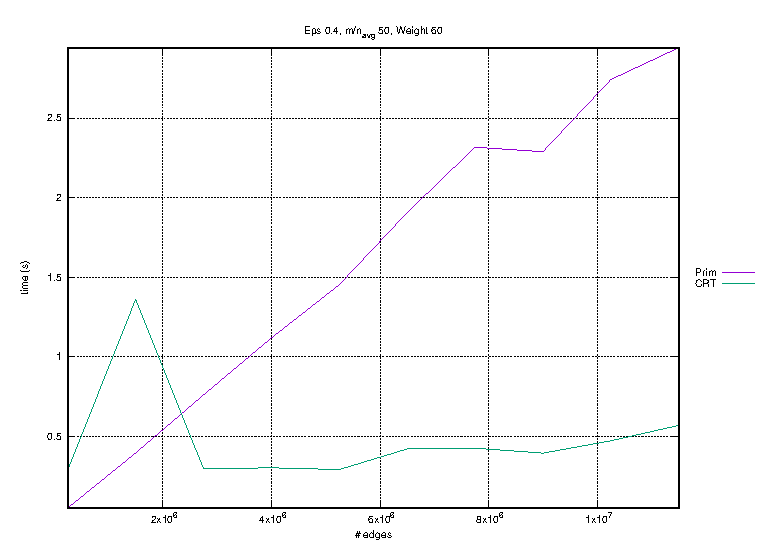
\includegraphics[width=.411\textwidth]{plots/gaussian_04_50_60_time}\label{G_04_50_60_time}}
 \subfloat[][small world, time trend]
 {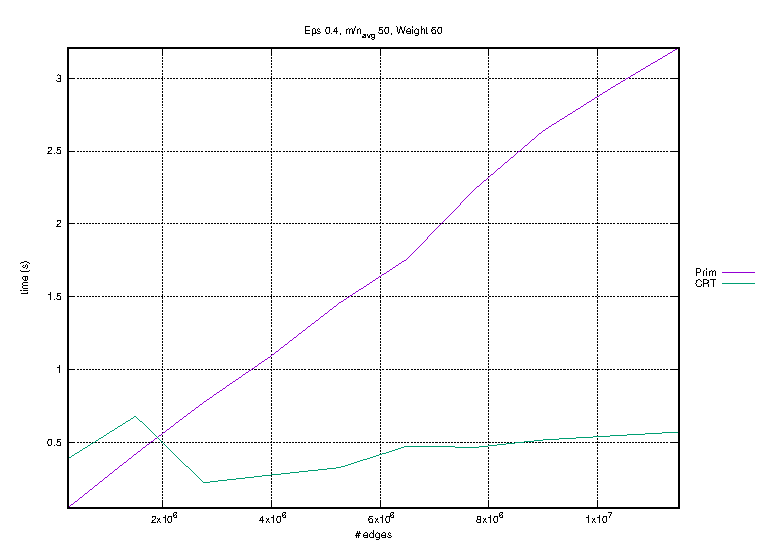
\includegraphics[width=.411\textwidth]{plots/smallworld_04_50_60_time}\label{SW_04_60_40_time}}
 \subfloat[][scale free, time trend]
 {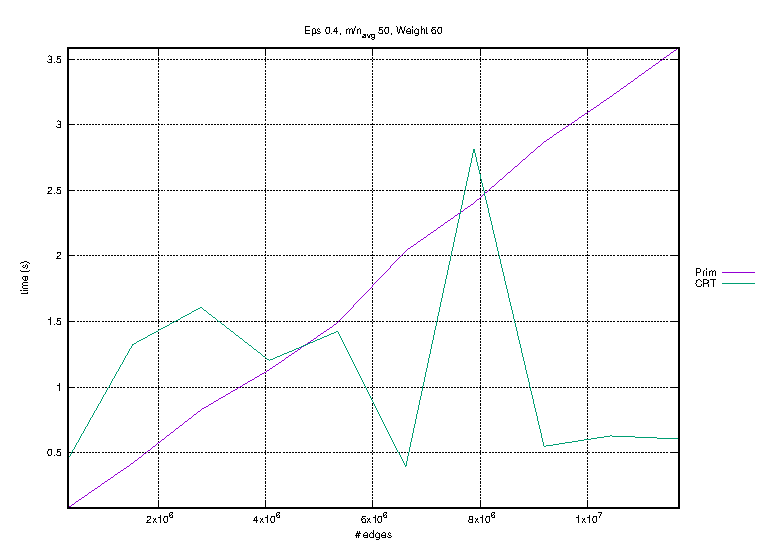
\includegraphics[width=.411\textwidth]{plots/scalefree_04_50_60_time}\label{SF_04_60_40_time}} \\
 \subfloat[][uniform, relative error]
 {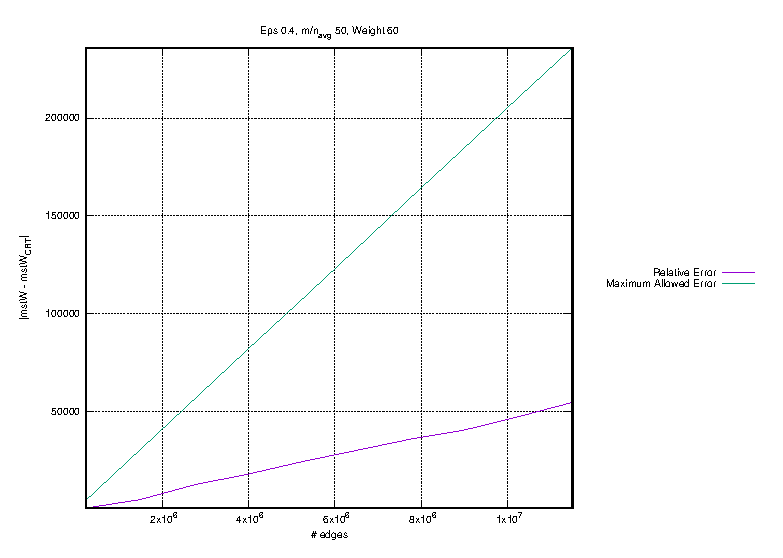
\includegraphics[width=.411\textwidth]{plots/uniform_04_50_60_rel}\label{U_04_50_60_rel}}
 \subfloat[][gaussian, relative error]
 {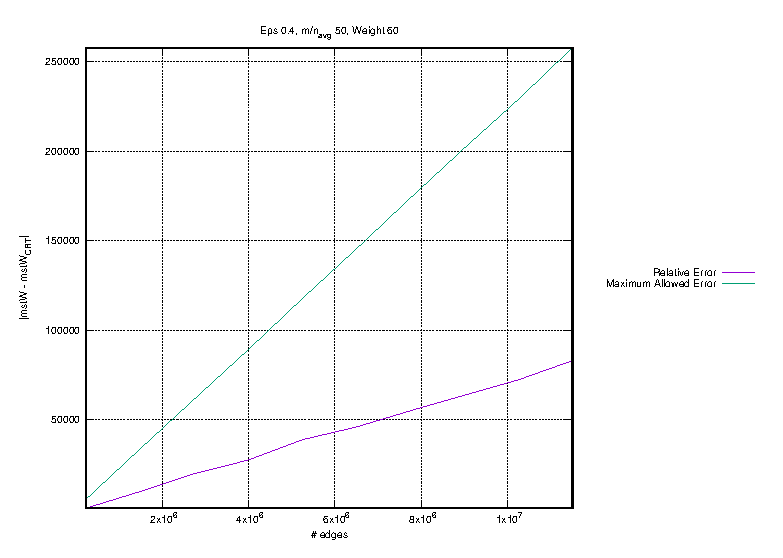
\includegraphics[width=.411\textwidth]{plots/gaussian_04_50_60_rel}\label{G_04_50_60_rel}}
 \subfloat[][small world, relative error]
 {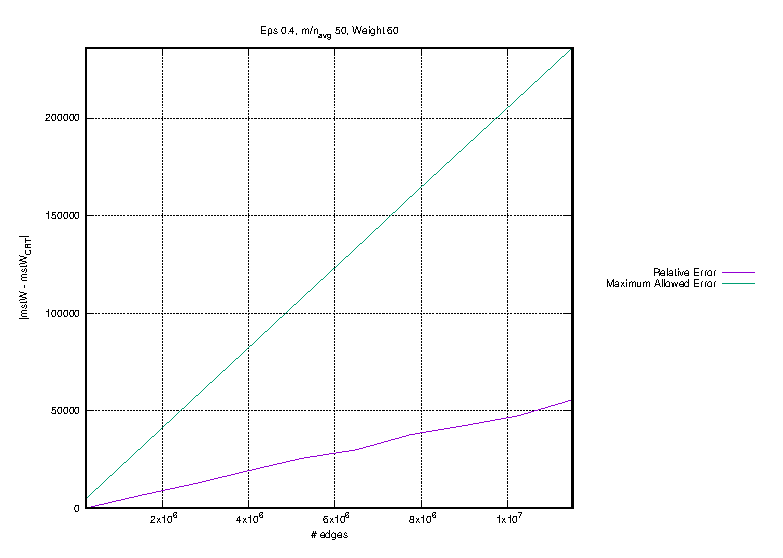
\includegraphics[width=.411\textwidth]{plots/smallworld_04_50_60_rel}\label{SW_04_50_60_rel}}
 \subfloat[][scale free, relative error]
 {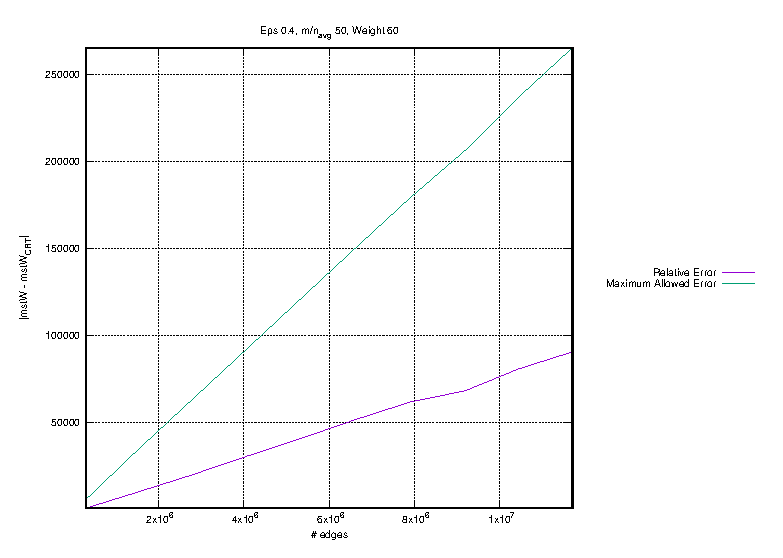
\includegraphics[width=.411\textwidth]{plots/scalefree_04_50_60_rel}\label{SF_04_50_60_rel}}
 \caption{Different behaviours for different graph models; fixed values are $\varepsilon = 0.4$, $\bar{d} = 50$, $w_\textup{max} = 60$.}
 \label{model_variation}
\end{figure}

\end{landscape}
 
While in the corresponding Small-World graph and the corresponding Uniform graph the trend is similar to the Gaussian graph (Fig.~\ref{GAUSSIAN_E_02_W_20_D_100}), in the Scale-Free case the reader can easily see that CRT algorithm takes a little 'more time' to down permanently under Prim execution time (Fig.~\ref{SCALE_FREE_E_02_W_20_D_100}). This can be related to the presence, in this kind of graph, of different nodes that have an high degree, which can make slower the execution. \\ The reader can also may notice that for small instances (few edges) the CRT algorithm is worse than deterministic algorithms, but when increasing the graph size the trend returns to be sub-linear again. \\Also comparing, for example, (Fig.~\ref{GAUSSIAN_E_02_W_20_D_100}) with the corresponding (Fig.~\ref{GAUSSIAN_E_02_W_20_D_10}), one can easily see that the performances become worse, as expected having increased the $d$ value. \\ 

Let us now see what happens if we increase $w$, keeping $d$ and $\varepsilon$ unchanged.
 

 
As expected, the CRT running time is higher than before. To be precise, what happens is that for the Gaussian, for the Scale-Free and for the Uniform the trend is about the same (Fig.~\ref{GAUSSIAN_E_02_W_80_D_100}), while for the Small-World case the reader can observe (Fig.~\ref{SMALL_WORLD_E_02_W_80_D_100}) that for large graph instances the trend becomes sublinear. We can imagine that the same happens for even larger instances also in the previous three kinds of graph.
 
To see if this is true we create an ad-hoc graphs dataset, that is an extension of our previously discussed dataset.\\
We generate an extension in the Uniform graphs dataset, adding larger instances (i.e. in terms of nodes and edges), and we want to see if the CRT algorithm becomes sub-linear, as expected, onwards from a certain point.


 

As the reader can see in Fig.~\ref{UNIFORM_BIG_RUN_EPS}, for larger instances the CRT algorithm really becomes sub-linear and its performances are better than, for example, Prim Algorithm.
\\

This is in agreement with the definition of the $O$ notation, that, for large arguments, indicates that the asymptotic behavior is of a certain type.\\

To conclude the discussion on the consistency of the execution time, we want now to see what happens in the case we increase $\varepsilon$, keeping $d$ and $w$ unchanged. \\Since the $\varepsilon$ parameter is a denominator for the estimated running time, what is expected is that an increase of this value corresponds to improved performances.

We can compare, for example, the performances of the CRT algorithm on two Small-World graphs with the following parameters: 
\begin{itemize}
\item $d=10$ 
\item $w=20$
\item and compare what happens for $\varepsilon=0.2$ and $\varepsilon=0.4$
\end{itemize}
 
 
 
 
The reader can easily see that the CRT trend has decreased.
 
 
 
 \section{Final thoughts} 
 
As expected, a probabilistic algorithm like the CRT allows us to compute an approximation of the Minimum Spanning Tree weight in sublinear time on the number of edges, under certain conditions.
Tunable parameters, that depends on $\varepsilon$, allows us to perform either a better or a worse approximation, implying respectively a very slow and a very fast computation. The choice of a small value of $\varepsilon$ can lead to terrible running times, and for these values it does not make sense to compare the CRT algorithm with any other deterministic algorithm.\\
For other $\varepsilon$ values, instead, we prove the good performances of the CRT. The reader can easily view the better performances of CRT algorithm versus Prim algorithm or Kruskal algorithm watching the line charts in the previous section of this paper.
 
\subsection{Parallel implementation}
We observe that the CRT algorithm lends itself very well to a parallel implementation. Indeed the majority of the algorithm's code is organized into independent sections, and in most cases they don't need to comunicate to each other. We also observe that three levels of paralellism can be achieved within the code. In the first level we parallelize each of the $w$ independent calls to \texttt{approx-number-connected-components}; every call internally performs $r$ independent BFSes from $r$ different roots, that could in turn run in parallel, achieving a second level of parallelism. Moreover, considering that in the academic world there already exist different parallel implementations of the BFS algorithm, we can use one of them to perform an additional third level of paralellism.

To make it even more simpler, the number of different flows is known a priori, so a static pre-instantiation and a smart scheduling of the threads can be performed. At the first and second levels a \emph{master-slave} model can be used in a \emph{fork-join} structure, while in the third level a shared variable is needed between the different BFSes. As a final remark, parallelizing the BFSes could have too much overhead given that the algorithm is optimized to run them very fast and to stop the ones that seem to cost too much.

\section{Future prospects}

During an e-mail exchange with one of the original authors of \cite{crt}, Dr. Ronitt Rubinfeld, another topic of discussion and study has emerged, about the distribution of the weight on the edges.

\begin{figure}[htbp]
 \centering
 \subfloat[][Assuming a uniform distribution]
 {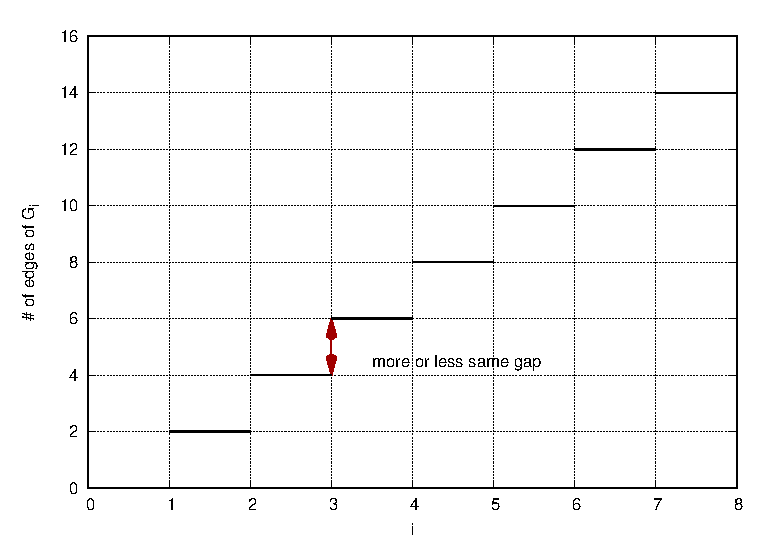
\includegraphics[width=.525\textwidth]{plots/same_gap}\label{same_gap}}
 \subfloat[][Assuming a generic distribution]
 {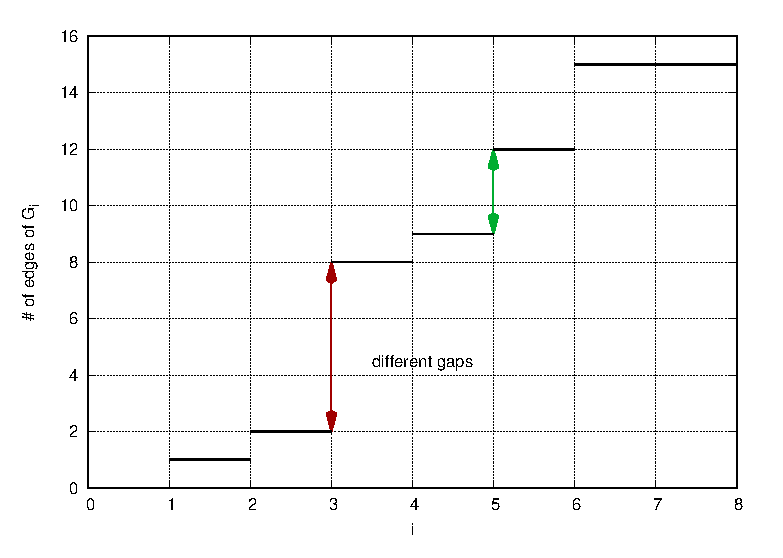
\includegraphics[width=.525\textwidth]{plots/diff_gap}\label{diff_gap}}
 \caption{Expected behaviour with different laws for the distribution of weights.}
 \label{gaps}
\end{figure}

In our code, the generation of random graphs only assume a uniform distribution of the weights on the edges, i.e. a given edge can have an integer weight $k \in [1, w]$ with probability $\frac{1}{w}$. That implies a linear growth of the dimension of $E(G_i), \forall i \in [1, w]$, namely the set of $G_i$'s edges; this is well depicted in figure~\cite{same_gap}, where, as $i$ grows, the size of $E(G_i)$ increases at each step of a quantity ``near'' $\frac{ \left| E(G) \right| }{w}$, and it is more true as $\left| E(G) \right|$ is big for the law of large numbers. On the other side, having a generic law of distribution for the edges weight implies having a different behavior as depicted on~\cite{diff_gap}.

This difference could be of interest because it means that the input of different subsequent iterations of \texttt{approx\_num\_connected\_comps} will have a non regularly increasing size, or even the same size for some calls; it can be easily shown indeed that the function in~\cite{gaps} is nondecreasing. Since the cost of those calls finally determines the overall cost, we might argue that this could lead to a minor difference, but at the same time think that only with another set of tests we could conclude something relevant about this observation.



%Another thing that we notice is that the algorithm lends well itself to a parallelized running; for example, we can easily make parallelized the execution of the “approx-MST-weight” routine, using $w-1$ threads. Since a parallel execution is out of scope to prove the algorithm goodness, this observation leads only to a possible future development; in this context, we are only interested in testing the sequential algorithm bound. VA SULLE CONSIDERAZIONI FINALI

 
 
\begin{thebibliography}{10}

\bibitem{crt} {\sc B. Chazelle, R. Rubinfeld, and L. Trevisan}, Approximating the minimum spanning tree weight in
sublinear time. SIAM J {\em Computing}, 34, 2005.

\bibitem{bst} {\sc Beman Dawes, David Abrahams, Rene Rivera}, Boost C++ Libraries. http://www.boost.org/.

\bibitem{fys} {\sc Fisher, Ronald A.; Yates, Frank (1948) [1938]}, Statistical tables for biological, agricultural and medical research (3rd ed.). London: Oliver \& Boyd. {\em pp. 26–27}.

\bibitem{fysc} {\sc Durstenfeld, R. (July 1964)}, ``Algorithm 235: Random permutation''. {\em Communications of the ACM}.

\end{thebibliography} 

\end{document} 

